\documentclass[tikz, border=12pt]{standalone}
\usepackage{tikz}
\usetikzlibrary{automata, positioning, arrows.meta, shapes.misc}
\usepackage{amsmath}
\begin{document}

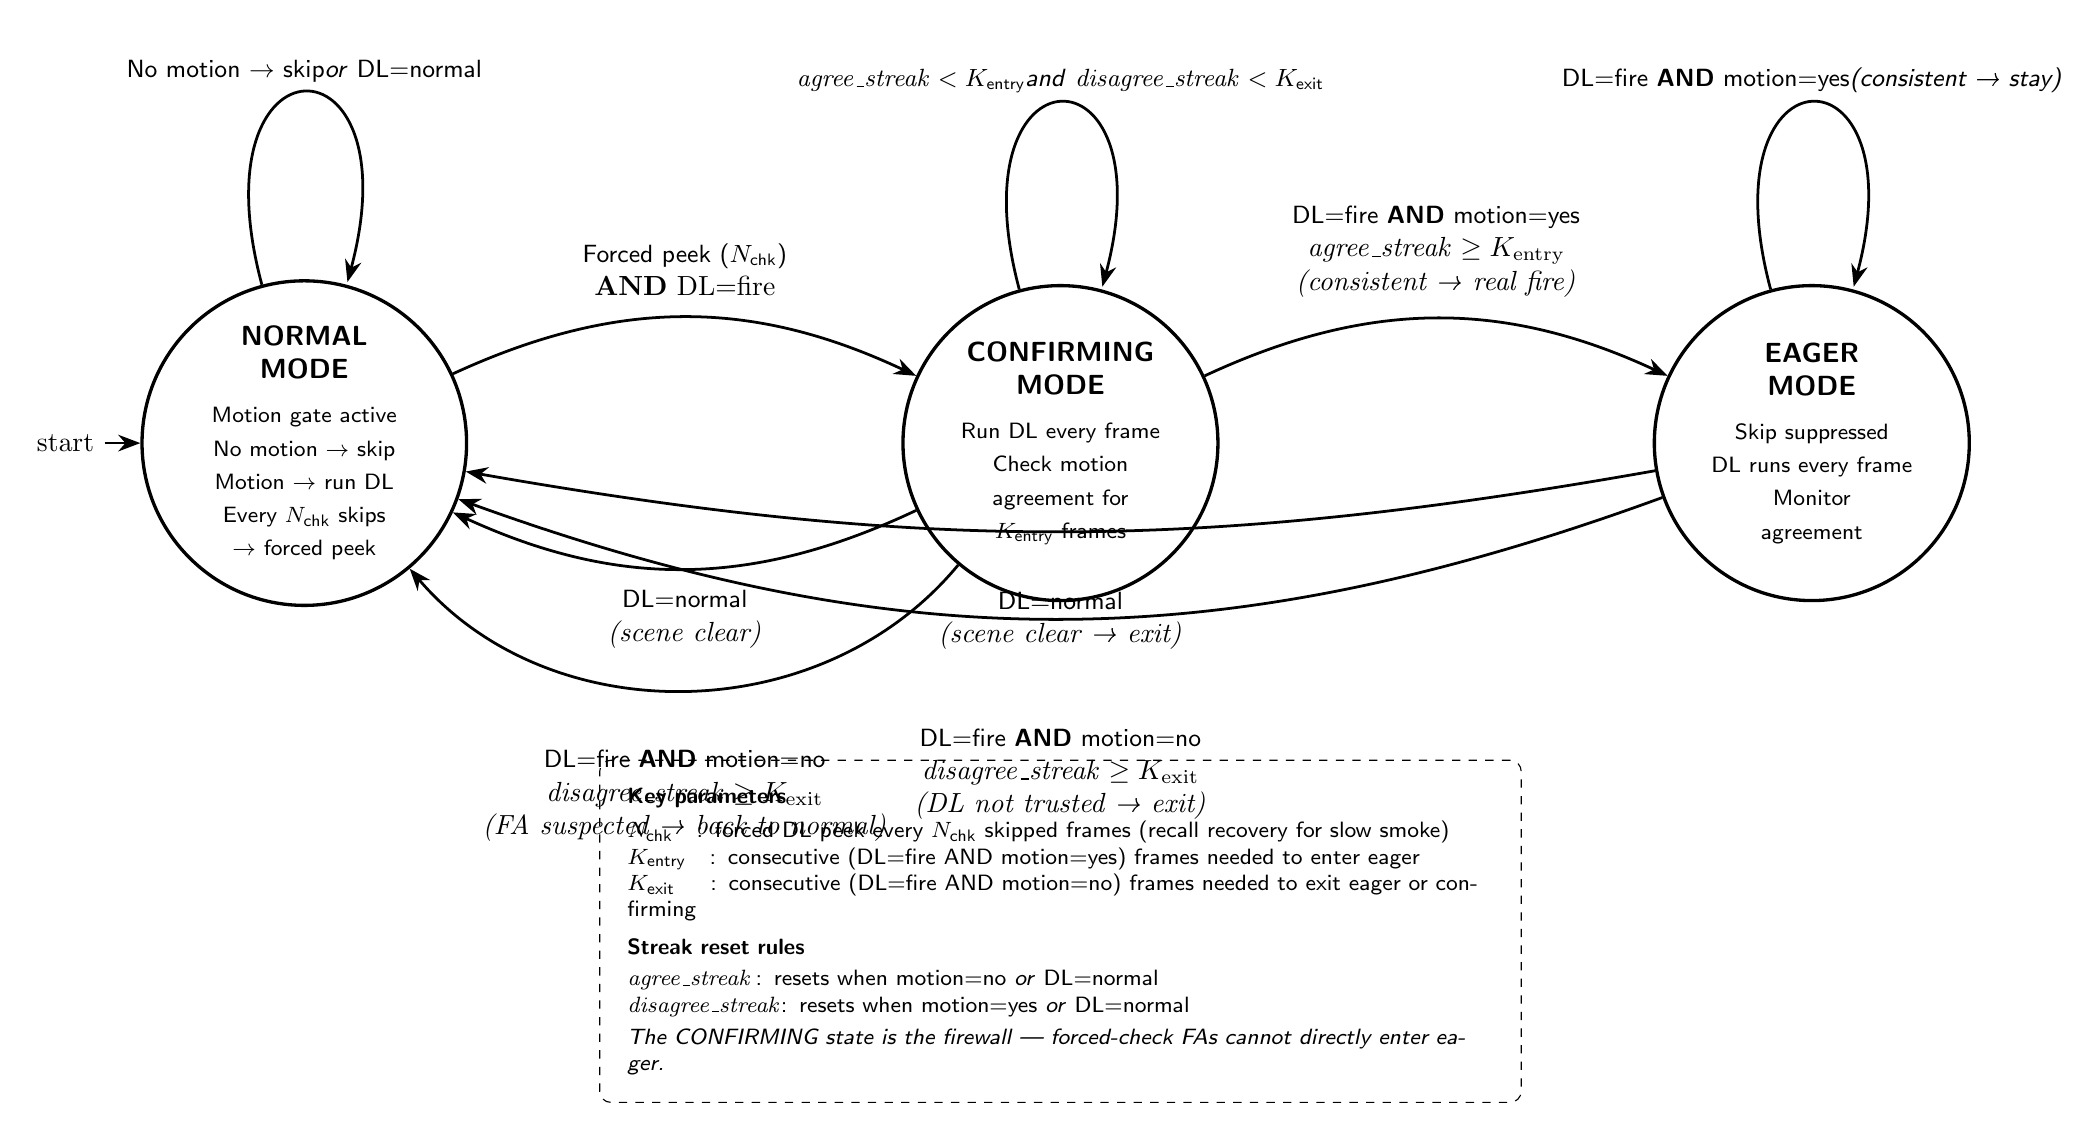
\begin{tikzpicture}[
    node distance=5.5cm,
    every state/.style={
        draw,
        rounded corners=8pt,
        minimum width=4.0cm,
        minimum height=3.0cm,
        align=center,
        font=\sffamily,
        line width=1.2pt
    },
    initial text={start},
    ->,
    >={Stealth[length=8pt]},
    every edge/.style={draw, line width=1pt},
    every edge quotes/.style={font=\sffamily\small, align=center}
]

%% ── States ───────────────────────────────────────────────────────────────────

\node[state, initial left] (normal)
    {\textbf{NORMAL}\\
     \textbf{MODE}\\[4pt]
     \footnotesize Motion gate active\\
     \footnotesize No motion $\rightarrow$ skip\\
     \footnotesize Motion $\rightarrow$ run DL\\
     \footnotesize Every $N_{\text{chk}}$ skips\\
     \footnotesize $\rightarrow$ forced peek};

\node[state, right=of normal] (confirm)
    {\textbf{CONFIRMING}\\
     \textbf{MODE}\\[4pt]
     \footnotesize Run DL every frame\\
     \footnotesize Check motion\\
     \footnotesize agreement for\\
     \footnotesize $K_{\text{entry}}$ frames};

\node[state, right=of confirm] (eager)
    {\textbf{EAGER}\\
     \textbf{MODE}\\[4pt]
     \footnotesize Skip suppressed\\
     \footnotesize DL runs every frame\\
     \footnotesize Monitor\\
     \footnotesize agreement};

%% ── NORMAL → CONFIRMING ──────────────────────────────────────────────────────
\draw (normal) edge[bend left=25]
    node[above, yshift=4pt, align=center]{%
        \sffamily\small
        Forced peek ($N_{\text{chk}}$)\\
        \textbf{AND} DL=fire}(confirm);

%% ── CONFIRMING → EAGER ───────────────────────────────────────────────────────
\draw (confirm) edge[bend left=25]
    node[above, yshift=4pt, align=center]{%
        \sffamily\small
        DL=fire \textbf{AND} motion=yes\\
        $\mathit{agree\_streak} \geq K_{\text{entry}}$\\
        \textit{(consistent → real fire)}}(eager);

%% ── CONFIRMING → NORMAL: DL says normal ─────────────────────────────────────
\draw (confirm) edge[bend left=25]
    node[below, yshift=-4pt, align=center]{%
        \sffamily\small
        DL=normal\\
        \textit{(scene clear)}}
    (normal);

%% ── CONFIRMING → NORMAL: disagree (FA suspected) ────────────────────────────
\draw (confirm) edge[bend left=50]
    node[below, yshift=-18pt, align=center]{%
        \sffamily\small
        DL=fire \textbf{AND} motion=no\\
        $\mathit{disagree\_streak} \geq K_{\text{exit}}$\\
        \textit{(FA suspected → back to normal)}}
    (normal);

%% ── EAGER → NORMAL: disagreement ────────────────────────────────────────────
\draw (eager) edge[bend left=20]
    node[below, yshift=-36pt, align=center]{%
        \sffamily\small
        DL=fire \textbf{AND} motion=no\\
        $\mathit{disagree\_streak} \geq K_{\text{exit}}$\\
        \textit{(DL not trusted → exit)}}
    (normal);

%% ── EAGER → NORMAL: DL says normal ──────────────────────────────────────────
\draw (eager) edge[bend left=10]
    node[below, yshift=-18pt, align=center]{%
        \sffamily\small
        DL=normal\\
        \textit{(scene clear → exit)}}
    (normal);

%% ── Self-loop EAGER: still agree ────────────────────────────────────────────
\draw (eager) edge[loop above]
    node[above]{%
        \sffamily\small
        DL=fire \textbf{AND} motion=yes\\
        \textit{(consistent → stay)}}
    (eager);

%% ── Self-loop NORMAL: skip / no trigger ─────────────────────────────────────
\draw (normal) edge[loop above]
    node[above]{%
        \sffamily\small
        No motion $\rightarrow$ skip\\
        \textit{or} DL=normal}
    (normal);

%% ── Self-loop CONFIRMING: still confirming ───────────────────────────────────
\draw (confirm) edge[loop above]
    node[above]{%
        \sffamily\small
        $\mathit{agree\_streak} < K_{\text{entry}}$\\
        \textit{and} $\mathit{disagree\_streak} < K_{\text{exit}}$}
    (confirm);

%% ── Legend / notes box ───────────────────────────────────────────────────────
\node[draw, dashed, rounded corners=4pt, font=\sffamily\footnotesize,
      align=left, below=2.0cm of confirm,
      inner sep=10pt, text width=11cm]
{%
    \textbf{Key parameters}\\[3pt]
    $N_{\text{chk}}$\quad : forced DL peek every $N_{\text{chk}}$ skipped frames (recall recovery for slow smoke)\\
    $K_{\text{entry}}$\quad : consecutive (DL=fire AND motion=yes) frames needed to enter eager\\
    $K_{\text{exit}}$\quad\, : consecutive (DL=fire AND motion=no) frames needed to exit eager or confirming\\[4pt]
    \textbf{Streak reset rules}\\[2pt]
    $\mathit{agree\_streak}$\,: resets when motion=no \emph{or} DL=normal\\
    $\mathit{disagree\_streak}$: resets when motion=yes \emph{or} DL=normal\\[2pt]
    \textit{The CONFIRMING state is the firewall — forced-check FAs cannot directly enter eager.}
};

\end{tikzpicture}

\end{document}